\documentclass{article}
\usepackage{arxiv}
\geometry{a4paper}
\AtBeginDocument{\newgeometry{textheight=9.1in,textwidth=6.35in,top=.75in,headheight=14pt,headsep=20pt,footskip=26pt}}
\usepackage[utf8]{inputenc}
\usepackage[T1]{fontenc}
\usepackage{microtype}
\usepackage{amsmath,amssymb}
\usepackage{booktabs}
\usepackage{graphicx}
\usepackage{longtable}
\usepackage{caption}
\usepackage[numbers,sort&compress]{natbib}
\usepackage[hidelinks]{hyperref}
\renewcommand{\headeright}{CS329 Project Report}
\renewcommand{\undertitle}{Project Implementation Report}
\renewcommand{\shorttitle}{Ambulance Dispatch under Limited Communication}
\captionsetup{font=small,labelfont=bf}
\graphicspath{{../results/full_20261121/report_plots/}{../results/improvements_20261121/weight_sensitivity/report_plots/}}
% Generated by build_report_assets.py from raw_results.csv and summary_metrics.csv.
\newcommand{\NScenarioSeeds}{30}
\newcommand{\NPolicyRuns}{3450}
\newcommand{\NWeightRuns}{1080}
\newcommand{\NMatchedScenarioGroups}{1170}
\newcommand{\MeanIncidentsPerScenario}{507.6}
\newcommand{\FullBIDServicePercent}{99.7}
\newcommand{\NoneBIDServicePercent}{80.9}
\newcommand{\FullNoneServiceDifferencePP}{18.8}
\newcommand{\LearnedBIDCostGapPercent}{1.1}
\newcommand{\LearnedBIDServicePercent}{99.7}
\newcommand{\OracleBIDCostGapPercent}{0.9}
\newcommand{\OracleBIDServicePercent}{99.8}
\newcommand{\DeviationMeanImprovement}{6.80}
\newcommand{\DeviationMeanCILow}{-8.67}
\newcommand{\DeviationMeanCIHigh}{49.80}
\newcommand{\DeviationMaximumObserved}{6.80}
\newcommand{\DeviationRelativeGainPercent}{0.09}
\newcommand{\BTwoQMeanCriticalResponseMinutes}{4.7}
\newcommand{\BTwoMeanCriticalResponseMinutes}{4.7}


\title{The Price of Decentralization in Ambulance Dispatch: Cooperative Coordination under Limited Communication and Unknown Demand}
\author{Lingala Hasini (24110186) \And Poladasu Tanmai (24110261) \And Manjula Reddyboina Triveni (24110295)\\[3pt]
Indian Institute of Technology Gandhinagar}
\date{CS329 Multi-Agent Systems}

\begin{document}
\maketitle

\begin{abstract}
An ambulance sent to one emergency also leaves the area it was covering. This project-review study asks how decentralized task allocation performs when ambulances share a cooperative objective but have limited communication and incomplete knowledge of spatial demand. We complete the proposal with an event-driven synthetic city simulator, nearest and criticality-weighted baselines, a centralized coverage-aware heuristic, and local bidding agents. The simulator models Poisson calls, deadlines, queueing, round-trip busy time, repositioning, and full, radius-limited, lossy, or absent peer communication. Agents learn zone rates online; an oracle condition provides an information reference. We report seven proposal experiment families and a separate one-factor sensitivity analysis of the three objective weights. Results include service before deadline, response time among served calls, coverage, utilization, duplicates, misses, communication, demand error, and signed empirical cost gaps to B3. B3 is a heuristic rather than a certified optimum, so the gap can have either sign. Seeds, configurations, code, raw CSVs, plots, and report tables are supplied for reproduction.
\end{abstract}

\keywords{multi-agent systems \and ambulance dispatch \and coordination \and communication \and online demand learning}

\section{Introduction}
Emergency dispatch must balance rapid response to the current call against preserving availability near future demand. Sending the nearest ambulance can reduce immediate travel while leaving its home region without coverage. Relocation and covering models capture this fleet-level trade-off \cite{church1974,brotcorne2003,maxwell2010}. Our project-review proposal extends the question to a cooperative multi-agent setting: what happens when agents observe local demand and coordinate through an imperfect message channel?

We model the fleet as a cooperative Markov game with private state, a public call signal, and optional peer messages \cite{littman1994,bernstein2002,oliehoek2016}. A market-inspired bid lets each ambulance estimate the shared cost of responding; communication loss can fragment the set of bids an agent observes \cite{smith1980,matignon2012}. The study compares that mechanism with simple dispatch rules and a stronger centralized reference. The original proposal, instructor feedback, and assigned project tasks are preserved in \texttt{docs/reference/}.

The instructor's correction is central to our evaluation: B3 is a Hungarian assignment and greedy-repositioning heuristic, not the optimum centralized policy. We therefore make no theoretical claim that a decentralized policy must have nonnegative price of decentralization. Instead, we report a signed empirical cost gap against B3. Negative values mean the tested policy had lower measured cost than this heuristic on those matched seeds; they do not establish a general guarantee.

The completed study contributes (i) a reproducible simulator and common team-cost implementation, (ii) four policies, four peer-communication regimes, and discounted online rate learning, (iii) paired experiments corresponding to the seven proposal factors plus an independent coefficient-sensitivity extension, and (iv) a restricted unilateral-deviation evaluation. The report remains a completion of the submitted project review, not a replacement topic.

\section{Problem Formulation}
Let $G=(V,E)$ be a connected weighted grid whose edge weights are travel minutes. Ambulance $i$ has current staging node $x_i$ and fixed home zone $h_i$; $\tau(x,z)$ is shortest-path travel time. Zone $z$ generates calls as a piecewise-constant Poisson process with rate $\lambda_z(t)$ calls/hour. A call $e=(\ell_e,K_e)$ has location $\ell_e$, criticality $K_e\in\{1,\ldots,5\}$, and a criticality-dependent deadline. The new-call signal is public to all policies, matching the proposal's observation tuple. Ambulance positions, status, and learned rates remain local unless messages convey them.

An ambulance is idle, responding, or repositioning. If dispatched from $x_i$, it travels to the call, remains on scene for $s$, and returns to its dispatch node. Thus its busy interval is $B_i(e)=2T_i(e)+s$, where $T_i(e)=\tau(x_i,\ell_e)$. A queued call's response feasibility includes its waiting time and requires scene arrival by its remaining deadline. Multiple commitments to one call consume each ambulance's busy time, but the first scene arrival resolves the call and later responders receive no additional service credit. Calls unresolved by their deadline are counted once as expired.

For idle set $I$, define $\operatorname{cov}(I,z)=\mathbf{1}[\min_{j\in I}\tau(x_j,z)\leq\theta]$ and $L_i(z;I)=\operatorname{cov}(I,z)-\operatorname{cov}(I\setminus\{i\},z)$. The implemented shared per-dispatch surrogate is
\begin{align}
R_i(e)&=B_i(e)\sum_{z\ne h_i}\lambda_z(t)L_i(z;I), &
D_i(e)&=B_i(e)\lambda_{h_i}(t),\\
c(e,i)&=\alpha K_eT_i^{\mathrm{resp}}+\beta R_i(e)+\gamma D_i(e), &
C(\pi)&=\sum_{(e,i)\in\mathcal D(\pi)}c(e,i)+\rho N_{\mathrm{expired}}.
\end{align}
Busy time is converted to hours when multiplied by call rates. $R_i$ charges non-home demand only where dispatch changes idle coverage from covered to uncovered; $D_i$ charges home-zone demand during absence even if a backup remains. The sets of zones are disjoint, so these two terms do not overlap. Every ambulance receives the same team reward $u_i=-C_{\mathrm{step}}$. This weighted surrogate has arbitrary model units and is not a clinical or monetary valuation.

The BID score uses the same $\alpha$, $\beta$, and $\gamma$ terms with locally available positions and rates. It is an approximate local score: it omits future action sequences and expiration penalties, and its view can be stale. The equality of terms resolves the proposal's mismatch between the common payoff and the home-demand bid term. B3 evaluates pairwise costs from a shared pre-allocation state; with multiple assignments, coverage charges can overlap. These limitations are why neither policy is presented as an exact optimizer.

\section{Methodology}
\subsection{City, demand, and event simulation}
The default city is a $5\times5$ grid with two-minute edges and precomputed all-pairs shortest paths. Incident tapes are generated before policy rollouts, so every policy in a paired seed sees the same arrivals, severity draws, initial placements, deadlines, and demand schedule. Zone arrivals follow independent Poisson processes. Demand can be uniform, concentrated at fixed hotspots, or shifted at the horizon midpoint; total rates are 2.5, 5, or 10 calls/hour. Severity follows the configured five-category distribution, with lower deadlines for higher criticality.

The discrete-event loop processes equal-time events in this order: complete trips, resolve scene arrivals, close learning bins and deliver updates, expire overdue calls, add new arrivals, then dispatch feasible queued calls and consider repositioning. A scene arrival exactly at a deadline is service because it is processed before expiry. Arrival generation stops at the declared horizon, while outstanding calls and trips are drained to finalize outcomes. Coverage and utilization integrate only through the arrival horizon. Responders return to their dispatch node after scene time; repositioning moves along a shortest path and makes that ambulance unavailable until its destination is reached.

\subsection{Policies and bidding protocol}
\textbf{B1} selects the nearest feasible idle ambulance. \textbf{B2} minimizes $\alpha K_eT_i^{\mathrm{resp}}$ over the same candidate set. Since the same positive $\alpha K_e$ multiplies every candidate for a given call, B1 and B2 have identical ordering and deterministic ambulance-ID tie-breaking. We preserve the proposal's definitions instead of inventing a different B2.

\textbf{B3} observes global positions and true demand rates. It forms pairwise assignment costs, uses a Hungarian assignment with dummy choices when the number of calls and available ambulances differ, and greedily repositions units to improve demand-weighted coverage. This is a centralized heuristic benchmark, not a certificate of global or dynamic optimality.

For \textbf{BID}, each eligible ambulance $i$ computes
\begin{align*}
J_i(e)=&\ \alpha K_eT_i^{\mathrm{resp}}
 +\beta B_i(e)\sum_{z\ne h_i}\widehat\lambda^i_zL_i(z;\widehat I_i)\\
&+\gamma B_i(e)\widehat\lambda^i_{h_i}.
\end{align*}
The agent sends its bid and state to reachable peers. It commits if its pair $(J_i,\mathrm{ID}_i)$ is lowest among bids it received, including its own; ties resolve by ascending ID. The simulator records every local commitment and does not centrally choose the BID winner. Full communication gives a common bid view and a single winner whenever a feasible responder exists. With fragmented views, several local minima may commit. A no-communication event still exposes the call signal, so a local minimum exists whenever an eligible agent exists; misses occur through deadline infeasibility or later capacity loss, not a missing winner timeout.

\subsection{Communication and demand learning}
\textbf{Full} communication has unlimited radius and no packet drops. \textbf{Radius-limited} communication permits directed packets only within a fixed shortest-path radius. \textbf{Lossy} communication has unlimited range but independently drops directed packets. \textbf{None} sends no inter-agent packets. Delivery latency is zero. The call signal is shared and is not counted as peer communication. BID messages include bids, status changes, and rate updates; sent counts record eligible directed attempts and delivered counts successful delivery. A dropped in-range packet counts as sent.

Each zone is assigned to the nearest fixed home-base sensor, ties by ambulance ID. Its owner observes arrivals in that zone even while busy. At hourly bin $b$, its estimate updates as
\[
\widehat\lambda_{z,b}=(1-\eta)\widehat\lambda_{z,b-1}+\eta N_{z,b}/\Delta,
\]
where $N_{z,b}$ is the observed count and $\Delta=1$ hour. Owners transmit estimates through the peer channel; receivers deduplicate by owner, zone, and bin. Learned BID acts on received estimates; oracle BID gets true rates, and B3 uses global true rates. The oracle is an information reference. B1/B2 do not use rate estimates in dispatch. Oracle BID still runs the learner and sends rate packets, so its communication count includes updates not needed for its bids.

\subsection{Outcomes and empirical comparison}
Service rate is calls reached by a responder before deadline divided by all generated calls; missed-call rate is expired calls over the same denominator. Response means include only served calls, so they are interpreted jointly with service and missed rates. Critical response restricts this mean to $K\ge4$. Demand-weighted coverage is the time-average fraction of true-rate mass in zones covered by at least one idle unit within $\theta$; it is an availability proxy, not a service guarantee. Utilization is busy ambulance-minutes divided by fleet size times arrival-horizon minutes and includes response, scene, return, and reposition time. Demand RMSE averages zone-rate errors over agents and learning-bin boundaries; oracle values are zero by construction.

For policy $\pi$ and matched seed $s$, the absolute and relative signed cost gaps are
\[
\Delta_C(\pi,B3;s)=C_\pi(s)-C_{B3}(s),\qquad
g_{B3}(\pi;s)=\frac{C_\pi(s)-C_{B3}(s)}{C_{B3}(s)}
\quad(C_{B3}(s)>0).
\]
The ratio is undefined when B3 cost is zero; the absolute difference remains defined. Because B3 is heuristic, this empirical comparator can be negative. Confidence intervals use 2,000 percentile-bootstrap resamples of paired scenario seeds, not incidents; we report descriptive intervals, not multiple-comparison-adjusted tests or causal claims.

\subsection{Experimental design and deviation check}
The proposal's seven experiments vary fleet size (3, 5, 7, 10), total demand (2.5, 5, 10/hour), demand pattern (uniform, hotspots, shifting), communication (four regimes), rate knowledge (learned/oracle), severity mix (three distributions), and the original joint $\beta$--$\gamma$ trade-off. The joint sweep keeps $\alpha=1$ and changes $\beta=\gamma$ together, so its effects are not separable. We add a distinct one-factor sensitivity study that independently varies $\alpha\in\{0.5,1,2\}$, $\beta\in\{4,8,16\}$, and $\gamma\in\{4,8,16\}$ with the other weights at defaults. Each level uses 20 paired seeds and the same default city/demand configuration. The original run contains \NPolicyRuns policy episodes; the weight extension adds \NWeightRuns.

For unilateral deviation, each of the five BID agents is changed in turn to the named time-only score $\alpha K_eT_i^{\mathrm{resp}}$ for the episode, while other agents remain BID on the same seed. The per-seed maximum positive decrease in team cost is summarized. This is a restricted empirical deviation check, not an equilibrium proof over arbitrary strategies.

\section{Results}
The original experiment batch contains seven proposal families, \NScenarioSeeds{} paired seeds per level, and matched exogenous arrival tapes. The signed gap and service summaries below are regenerated directly from its raw records. Table~\ref{tab:proposal-results} gives the BID and B3 service means and the BID signed cost gap for every proposal level; negative gaps are retained. Communication outcomes are also reported with duplicate and missed-call rates because conditional response means alone can conceal failures.

\begin{figure}[t]
\centering
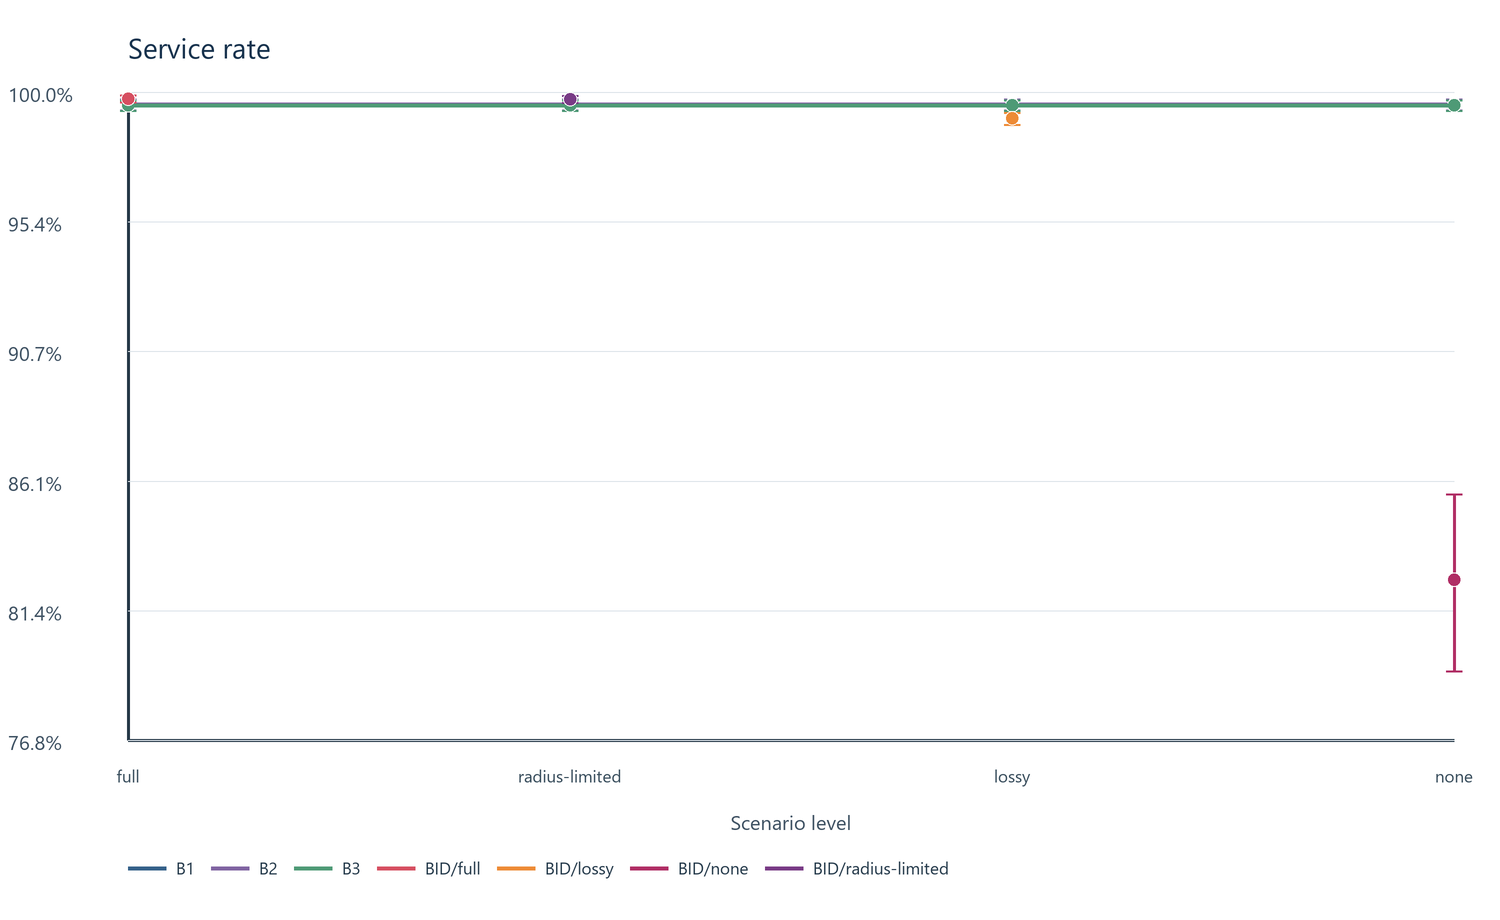
\includegraphics[width=.48\linewidth]{exp4_communication_service_rate.png}\hfill
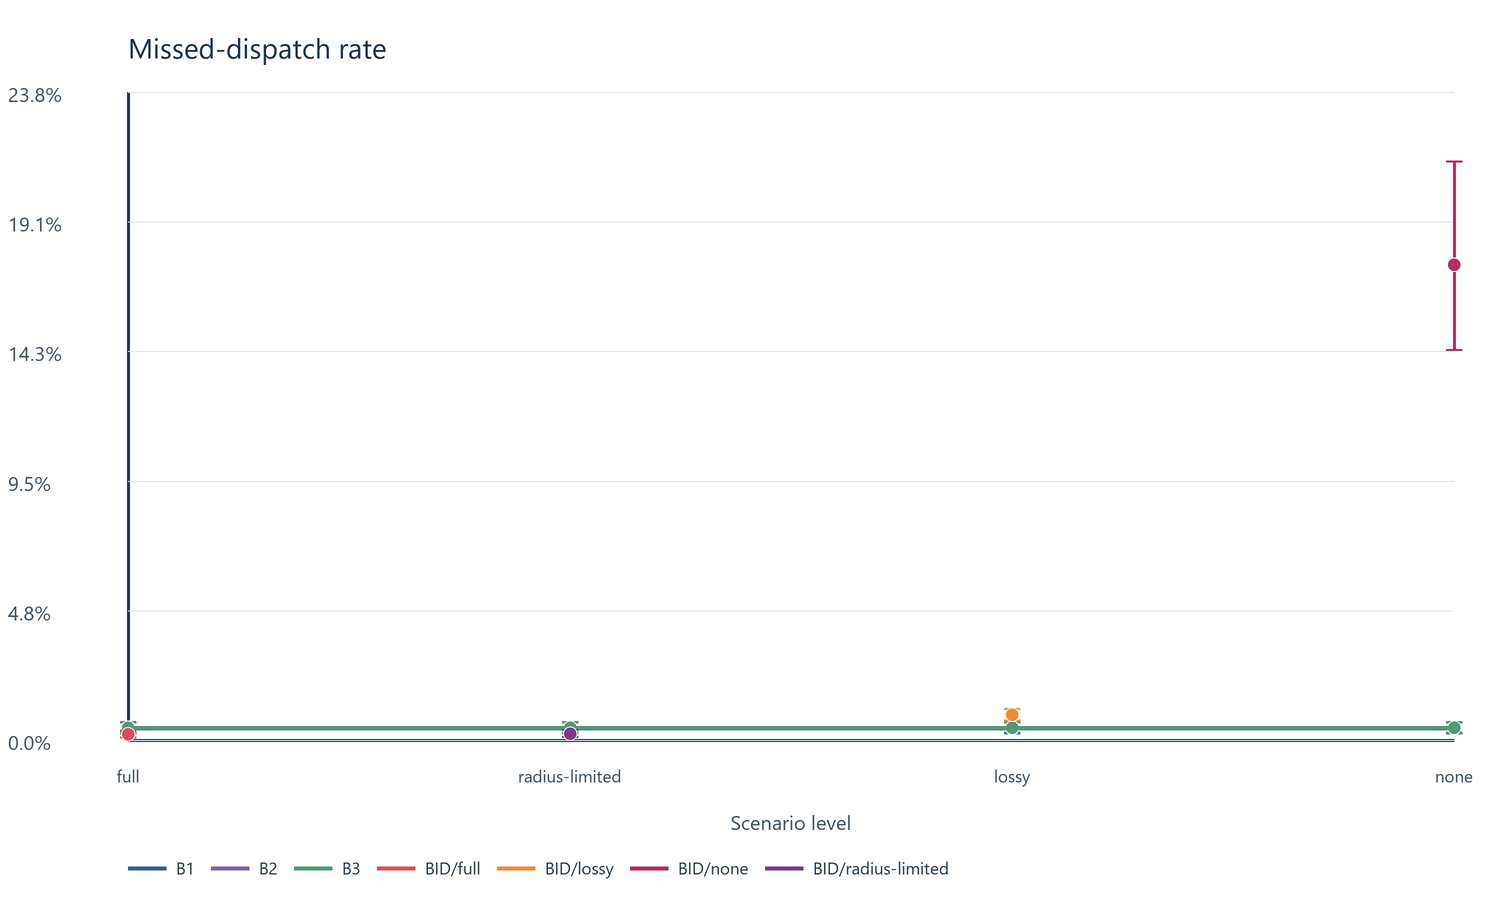
\includegraphics[width=.48\linewidth]{exp4_communication_missed_dispatch_rate.png}\\[-2pt]
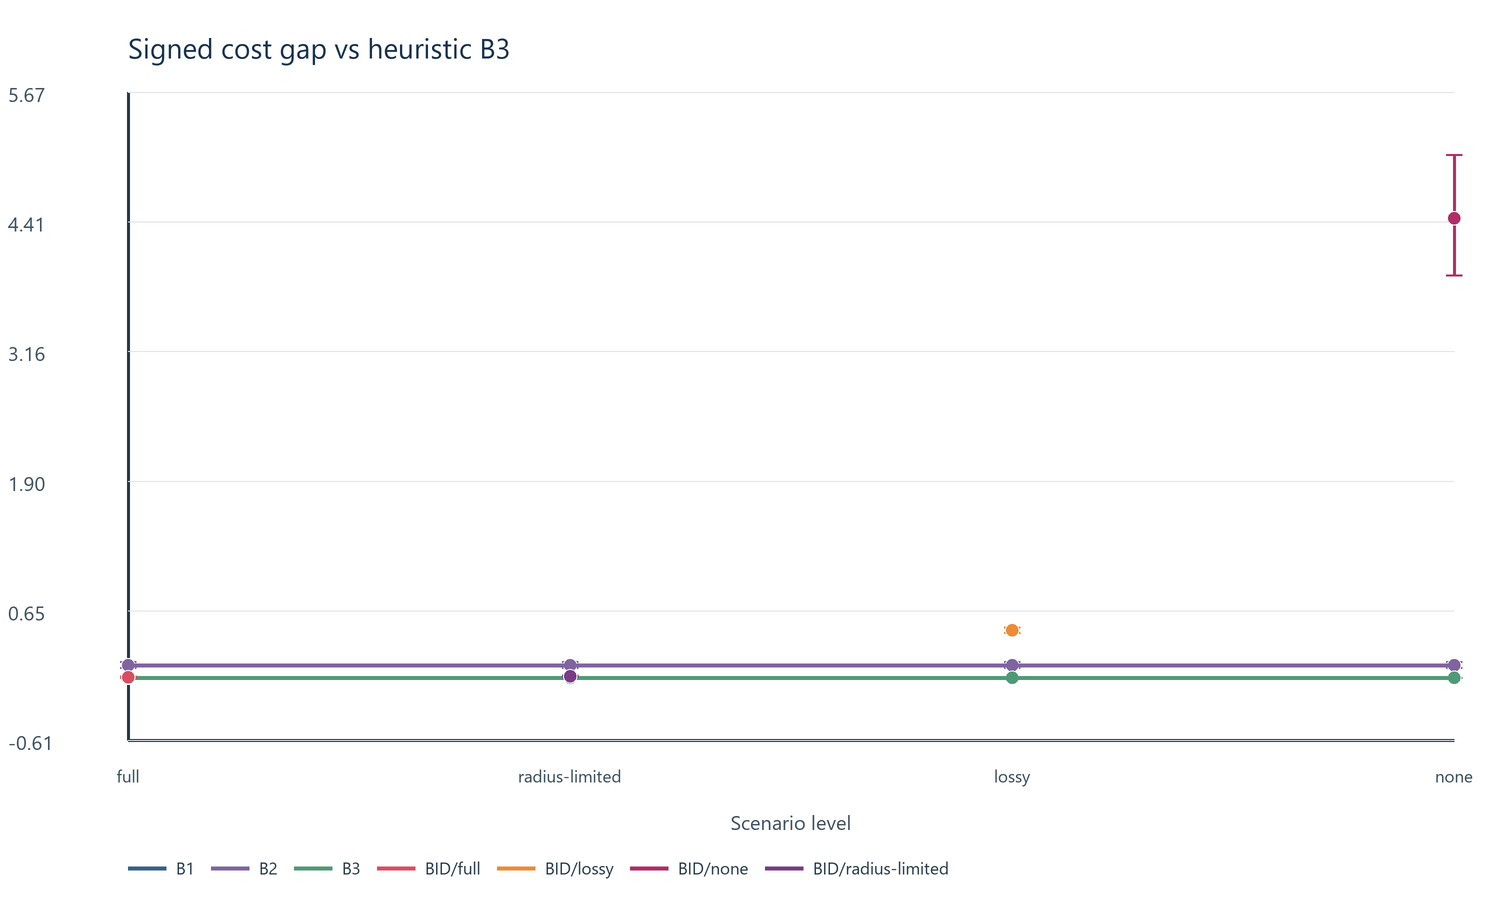
\includegraphics[width=.48\linewidth]{exp4_communication_b3_cost_gap_relative.png}\hfill
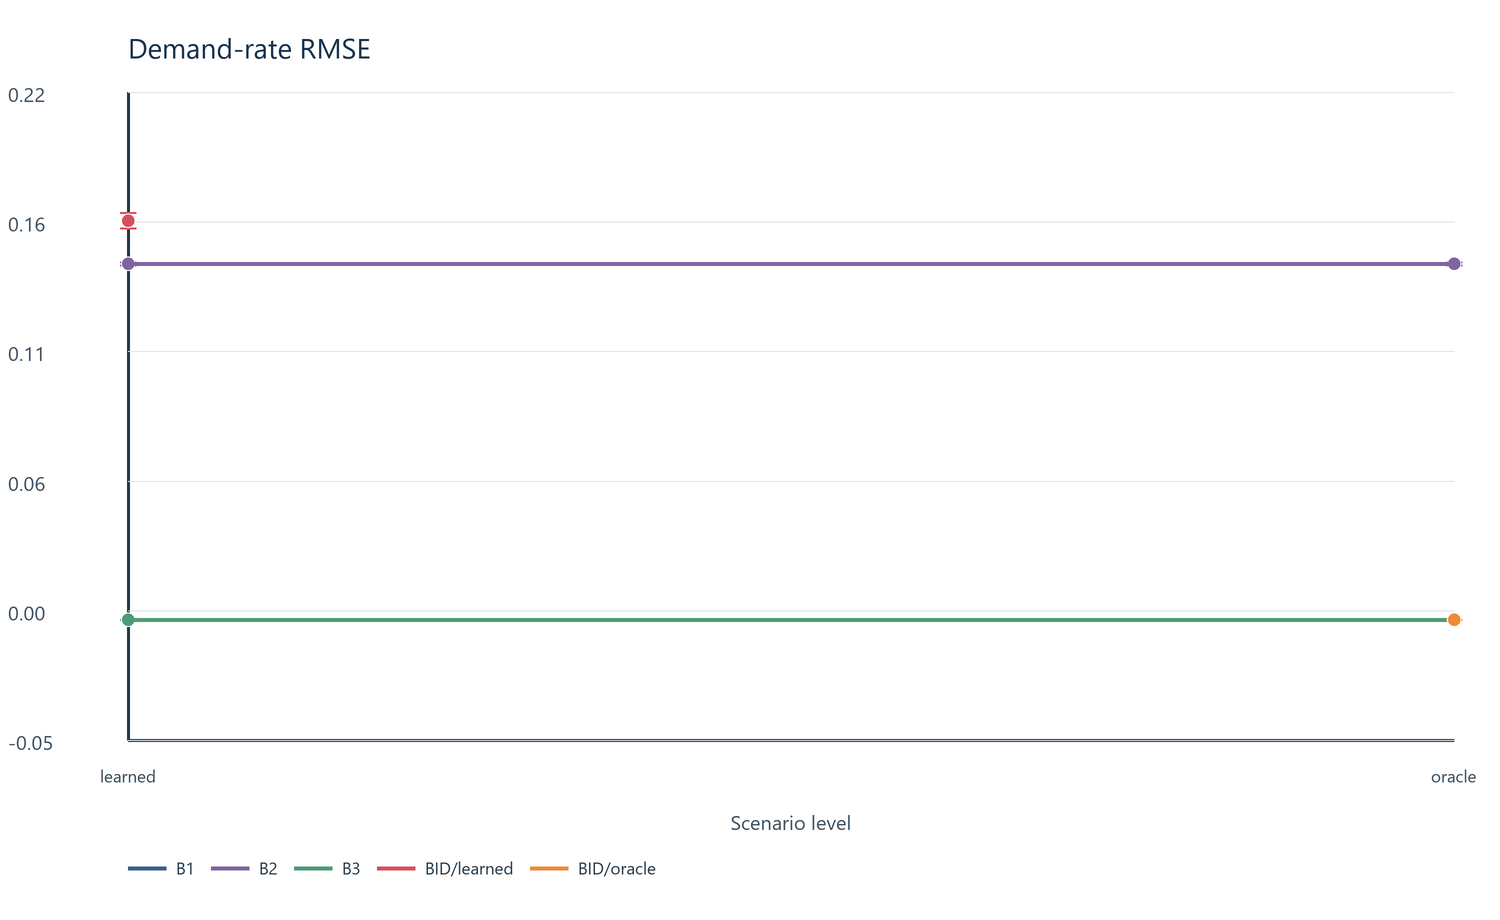
\includegraphics[width=.48\linewidth]{exp5_demand_knowledge_demand_rmse.png}
\caption{Communication and knowledge outcomes from the original proposal sweeps. Response outcomes are service before deadline; relative cost gaps are signed versus heuristic B3.}
\label{fig:communication-learning}
\end{figure}

Across the communication sweep, BID's full-versus-none service difference is \FullNoneServiceDifferencePP{} percentage points on average across paired seeds. The no-message condition also has the highest duplicate and missed-call means (Table~\ref{tab:communication-rates}). This pattern is consistent with multiple local minima consuming capacity, but the synthetic design does not isolate that mechanism causally. Radius-limited and lossy cases show that an imperfect view is not equivalent to full isolation.

The joint communication outcomes show why service should not be interpreted alone. No communication coincides with zero peer-message traffic, lower idle coverage, higher utilization, more duplicate commitments, and longer mean response among the calls that were served. Since missed calls are excluded from response means, that conditional statistic can conceal poor system performance; the table reports it beside service and missed-call rates. Full and radius-limited communication have closely aligned outcomes in this fixed setup, while packet loss produces an intermediate pattern. These are observed associations in paired synthetic scenarios, not a causal estimate of a universal communication benefit.

Demand knowledge yields similar average BID cost gaps in the configured learned and oracle conditions: \LearnedBIDCostGapPercent\% and \OracleBIDCostGapPercent\%, respectively. These small differences in the aggregate do not demonstrate that online learning is unnecessary; the default setup, estimator, objective, and \NScenarioSeeds{}-seed design limit that conclusion. B3 and oracle BID RMSE are zero by construction, while learned-policy errors are diagnostic estimates against the simulator's known rates.

The high-demand and three-ambulance rows in Table~\ref{tab:proposal-results} show lower service than the well-resourced conditions. The spatial-pattern and criticality sweeps change the scenario mix but do not establish a general ranking outside these fixed synthetic settings. B1 and B2 are exactly the same rule under their proposal definitions, which the \NMatchedScenarioGroups{} original matched groups confirm. In experiment 7, BID's gap varies with the joint $\beta$--$\gamma$ scaling; this cannot be attributed to either weight independently.

\begin{figure}[t]
\centering
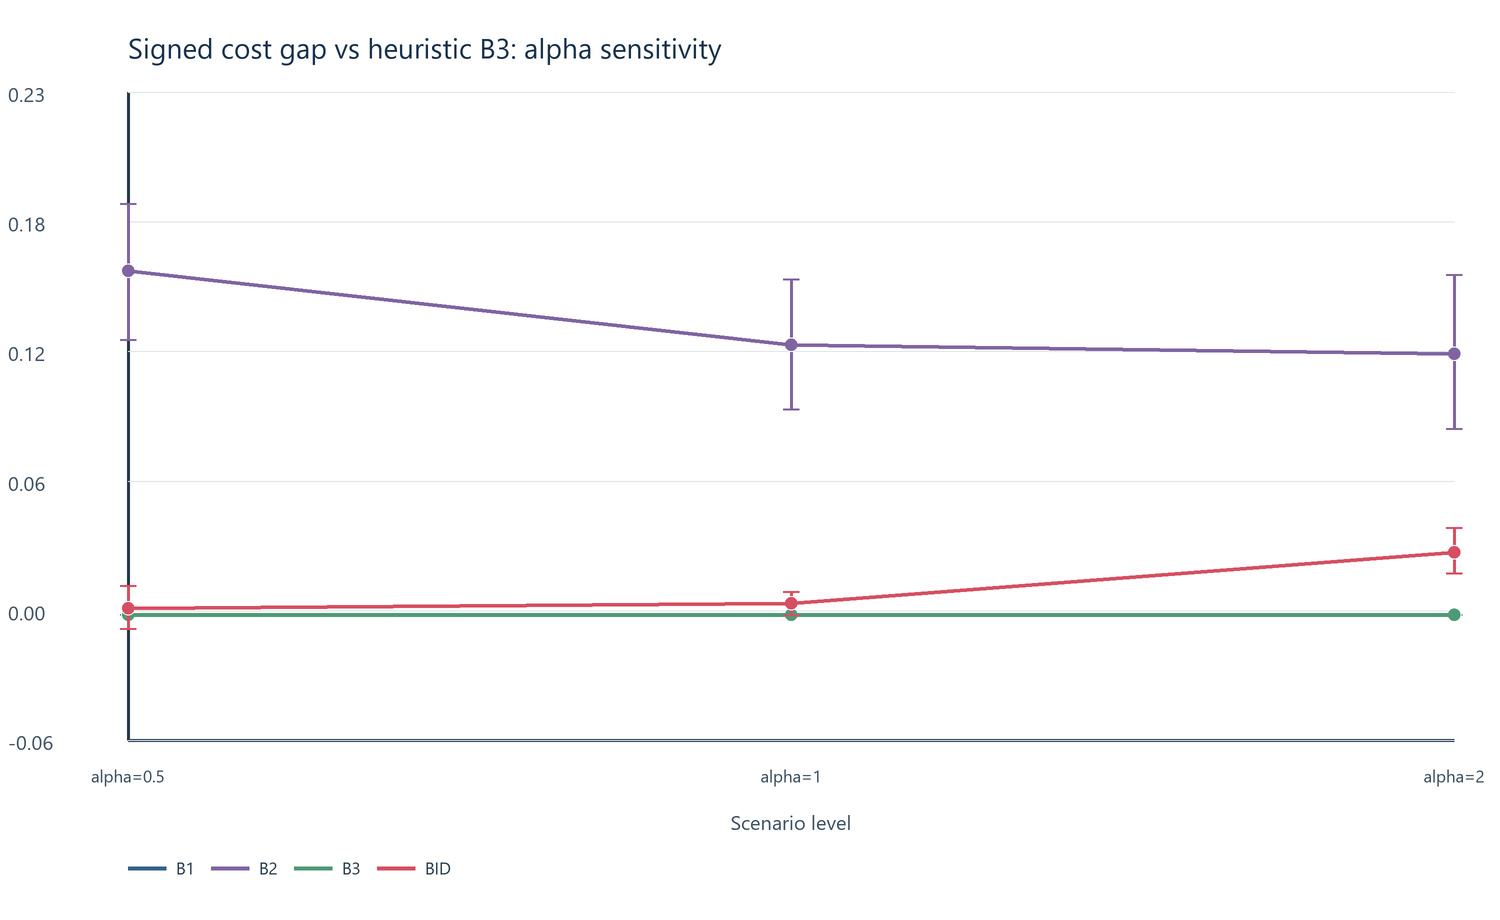
\includegraphics[width=.48\linewidth]{exp8_weight_sensitivity_alpha_b3_cost_gap_relative.png}\hfill
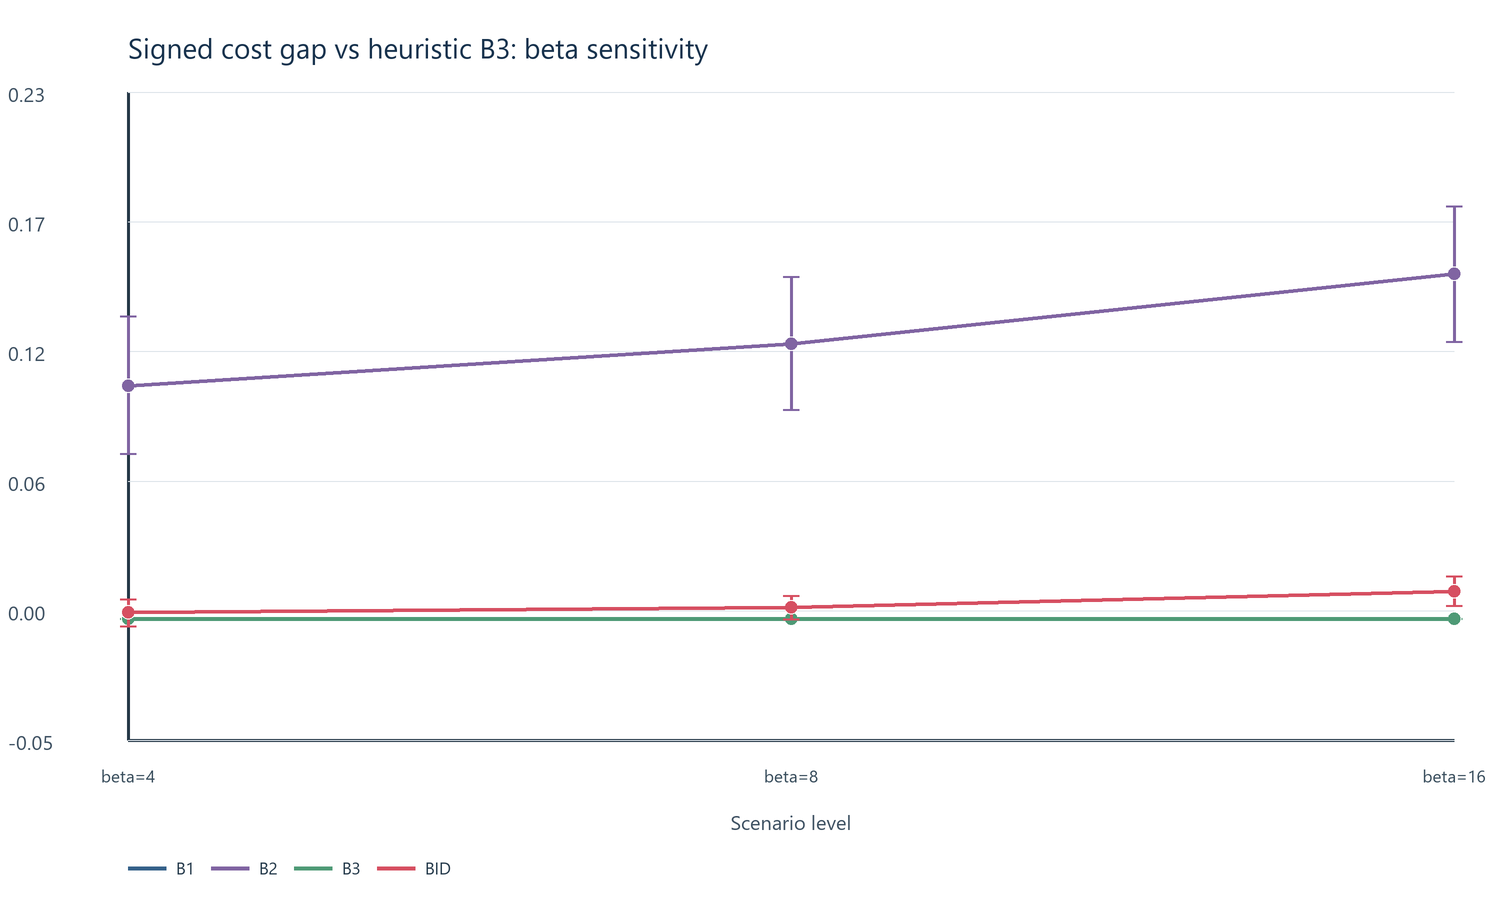
\includegraphics[width=.48\linewidth]{exp8_weight_sensitivity_beta_b3_cost_gap_relative.png}\\[-2pt]
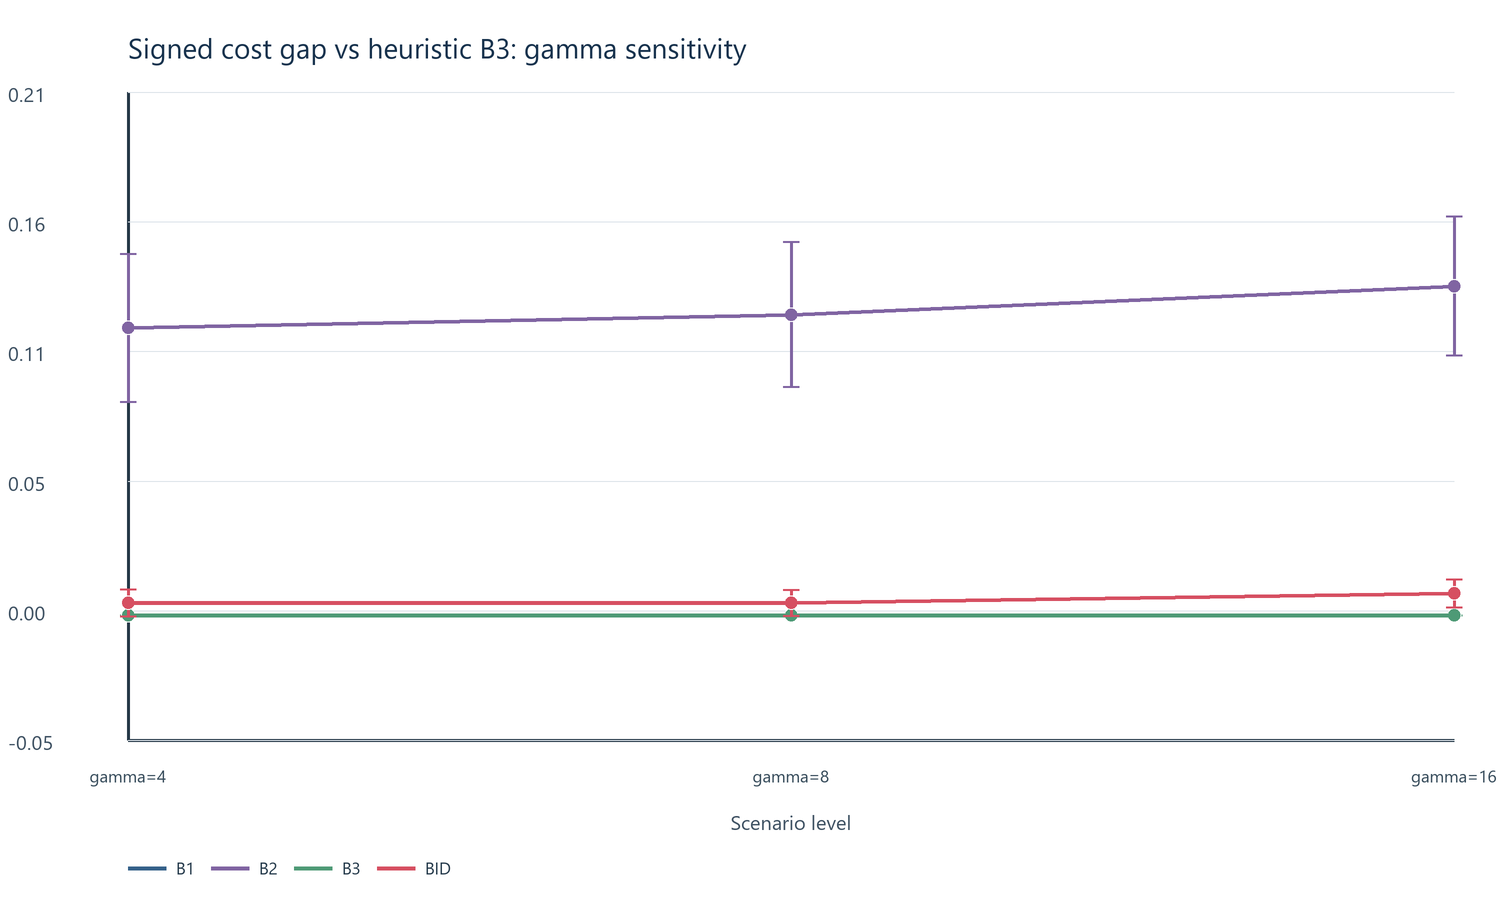
\includegraphics[width=.48\linewidth]{exp8_weight_sensitivity_gamma_b3_cost_gap_relative.png}
\caption{Additional independent sensitivity results for $\alpha$, $\beta$, and $\gamma$. Each coefficient changes alone; other weights remain at default. Points and intervals are seed-level BID gaps to B3.}
\label{fig:weight-sensitivity}
\end{figure}

The independent sensitivity batch has \NWeightRuns{} episodes (nine weight levels, four policies, \NScenarioSeeds{} seeds). Its service and signed-gap intervals are listed in Table~\ref{tab:weight-sensitivity}. This extension separates the coefficients that experiment 7 changed together. It remains a one-factor analysis: it does not estimate interactions, select globally optimal weights, or replace the originally proposed experiment.

\begin{table}[t]
\centering\scriptsize
\setlength{\tabcolsep}{3pt}
\caption{Proposal experiment results. Service and relative cost gap show mean [95\% paired-seed bootstrap interval]. The relative cost gap is signed versus heuristic B3.}
\label{tab:proposal-results}
\begin{tabular}{p{1.47in}p{1.47in}p{1.47in}p{1.47in}}
\toprule
Experiment level & BID service (\%) & B3 service (\%) & BID cost gap to B3 (\%) \\
\midrule
E1 Fleet, n=3 & 93.9\% [93.0,94.7] & 91.6\% [90.6,92.5] & 8.1\% [7.3,8.9] \\
E1 Fleet, n=5 & 99.8\% [99.6,99.9] & 99.5\% [99.3,99.7] & 0.5\% [-0.0,1.1] \\
E1 Fleet, n=7 & 100.0\% [100.0,100.0] & 100.0\% [99.9,100.0] & 3.3\% [1.1,6.1] \\
E1 Fleet, n=10 & 100.0\% [100.0,100.0] & 100.0\% [100.0,100.0] & 11.1\% [4.3,18.5] \\
E2 Demand, low:2.5/h & 100.0\% [100.0,100.0] & 100.0\% [100.0,100.0] & 4.5\% [1.5,7.3] \\
E2 Demand, medium:5/h & 99.8\% [99.6,99.9] & 99.5\% [99.3,99.7] & 0.5\% [-0.0,1.1] \\
E2 Demand, high:10/h & 93.1\% [92.6,93.7] & 90.5\% [90.0,91.0] & 16.0\% [15.0,17.0] \\
E3 Pattern, uniform & 99.5\% [99.4,99.7] & 99.3\% [99.1,99.4] & 0.3\% [-0.2,0.9] \\
E3 Pattern, hotspots & 99.8\% [99.6,99.9] & 99.5\% [99.3,99.7] & 0.5\% [-0.0,1.1] \\
E3 Pattern, shifting & 99.6\% [99.5,99.7] & 99.2\% [99.1,99.4] & 1.0\% [0.6,1.5] \\
E4 Communication, full & 99.8\% [99.6,99.9] & 99.5\% [99.3,99.7] & 0.5\% [-0.0,1.1] \\
E4 Communication, radius-limited & 99.8\% [99.6,99.9] & 99.5\% [99.3,99.7] & 1.3\% [0.7,2.1] \\
E4 Communication, lossy & 99.1\% [98.8,99.3] & 99.5\% [99.3,99.7] & 45.9\% [43.2,48.5] \\
E4 Communication, none & 82.5\% [79.2,85.6] & 99.5\% [99.3,99.7] & 444.7\% [389.5,506.2] \\
E5 Knowledge, learned & 99.8\% [99.6,99.9] & 99.5\% [99.3,99.7] & 0.5\% [-0.0,1.1] \\
E5 Knowledge, oracle & 99.8\% [99.7,99.9] & 99.5\% [99.3,99.7] & 0.4\% [-0.1,0.9] \\
E6 Criticality, low-heavy & 99.9\% [99.8,100.0] & 99.7\% [99.6,99.8] & 0.8\% [0.2,1.4] \\
E6 Criticality, balanced & 99.6\% [99.4,99.7] & 99.3\% [99.1,99.5] & 0.6\% [0.2,1.0] \\
E6 Criticality, high-heavy & 99.1\% [98.9,99.4] & 98.9\% [98.6,99.2] & 0.8\% [0.3,1.4] \\
E7 Weights, coverage-light & 99.8\% [99.6,99.9] & 99.5\% [99.3,99.7] & 0.1\% [-0.5,0.7] \\
E7 Weights, balanced & 99.8\% [99.6,99.9] & 99.5\% [99.3,99.7] & 0.5\% [-0.0,1.1] \\
E7 Weights, coverage-heavy & 99.8\% [99.6,99.9] & 99.5\% [99.3,99.7] & 1.6\% [0.8,2.4] \\
\bottomrule
\end{tabular}
\end{table}

\begin{center}
\scriptsize
\setlength{\tabcolsep}{2.5pt}
\captionof{table}{BID communication outcomes (means across 30 paired seeds). Response is conditional on service; message count is directed attempts per incident.}
\label{tab:communication-rates}
\begin{tabular}{lrrrrrrr}
\toprule
Regime & Service (\%) & Response (min) & Coverage (\%) & Util. (\%) & Msg./call & Duplicate (\%) & Expired (\%) \\
\midrule
full & 99.7 & 4.5 & 90.0 & 46.4 & 34.4 & 0.0 & 0.3 \\
radius-limited & 99.7 & 4.5 & 89.8 & 46.6 & 34.3 & 0.1 & 0.3 \\
lossy & 99.1 & 5.5 & 78.3 & 56.0 & 34.9 & 20.0 & 0.9 \\
none & 80.9 & 17.1 & 21.0 & 88.2 & 0.0 & 41.1 & 19.1 \\
\bottomrule
\end{tabular}
\end{center}

\begin{center}
\scriptsize
\captionof{table}{Independent one-factor weight sensitivity. Other weights remain at the default while each listed coefficient varies. Cells show mean [95\% paired-seed bootstrap interval].}
\label{tab:weight-sensitivity}
\setlength{\tabcolsep}{3pt}
\begin{tabular}{lrrr}
\toprule
Weight & Level & BID service (\%) & BID signed gap to B3 (\%) \\
\midrule
alpha & 0.5 & 99.7\% [99.6,99.8] & 0.2\% [-0.5,0.9] \\
alpha & 1 & 99.7\% [99.7,99.8] & 1.1\% [0.4,1.9] \\
alpha & 2 & 99.7\% [99.7,99.8] & 3.2\% [2.2,4.3] \\
beta & 4 & 99.7\% [99.6,99.8] & 0.7\% [0.1,1.5] \\
beta & 8 & 99.7\% [99.7,99.8] & 1.1\% [0.4,1.9] \\
beta & 16 & 99.8\% [99.7,99.8] & 1.6\% [1.0,2.2] \\
gamma & 4 & 99.7\% [99.7,99.8] & 1.1\% [0.4,1.9] \\
gamma & 8 & 99.7\% [99.7,99.8] & 1.1\% [0.4,1.9] \\
gamma & 16 & 99.7\% [99.6,99.8] & 1.4\% [0.7,2.1] \\
\bottomrule
\end{tabular}
\end{center}


\section{Unilateral Deviation and Contributions}
Across \NScenarioSeeds{} seeds under full communication, the maximum tested positive team-cost improvement averaged \DeviationMeanImprovement{} (95\% bootstrap interval [\DeviationMeanCILow, \DeviationMeanCIHigh]); the largest per-seed maximum was \DeviationMaximumObserved. A positive value means the tested time-only deviator reduced common cost relative to all-BID. Because only one named action change is evaluated per agent, the result is not a Nash or approximate-Nash certificate.

Table~\ref{tab:contributions} lists the original assignments from the proposal and the status of corresponding project deliverables. Repository inspection can verify that artifacts exist, but cannot establish which member personally completed or authored them. For this reason, the table does not assert individual completion or authorship without confirmation.

\begin{table}[h]
\centering\small
\setlength{\tabcolsep}{4pt}
\caption{Original proposal assignments and repository-verifiable status.}
\label{tab:contributions}
\begin{tabular}{p{1.1in}p{3.5in}p{1.4in}}
\toprule
Member & Originally assigned tasks (proposal wording condensed) & Evidence status \\
\midrule
Poladasu Tanmai & City, Poisson arrivals, criticality/deadlines, queues/busy times, B1/B2, Introduction, Preliminaries & Deliverables present; personal status unknown \\
Lingala Hasini & Decentralized bidding, four communication regimes, demand learning/oracle comparison, Problem Formulation, Proposed Solutions & Deliverables present; personal status unknown \\
Manjula Reddyboina Triveni & B3, experiment runner, metrics, B3 gaps, unilateral deviation, plots/results, Evaluation, Limitations & Deliverables present; personal status unknown \\
\bottomrule
\end{tabular}
\end{table}

\section{Discussion, Limitations, and Conclusion}
The simulator makes the proposed coordination trade-off measurable under controlled, paired scenarios. Communication conditions alter the BID agents' view of bids, state, and rate updates, while the public call signal remains common. In the no-message case, local minima can create duplicates; additional busy ambulances can reduce later capacity. The result is specific to the implemented protocol and should not be read as the effect of communication in every dispatch system.

The model has important limits. The city and arrival rates are synthetic; travel is deterministic, with no traffic, hospital destination, heterogeneous vehicle, delayed message, or real dispatch data. Calls shift once at the horizon midpoint. Return-to-dispatch-node travel and the common weighted surrogate simplify operational and clinical costs. Coverage is an idle-unit availability proxy. The rate learner is a fixed discounted estimator. B3 uses a shared snapshot and greedy repositioning rather than exact dynamic optimization. Oracle BID continues to exchange learner messages. Only one restricted unilateral deviation is tested. \NScenarioSeeds{} seeds and many factor-level comparisons support descriptive estimates, not broad causal or population claims.

The one-factor extension helps separate the proposal's joint weight sweep. Across the tested endpoints, the mean signed gap grows most in the $\alpha$ sweep, with smaller increases in the $\beta$ and $\gamma$ sweeps; BID service is effectively unchanged at the table's displayed precision (Table~\ref{tab:weight-sensitivity}). These are descriptive comparisons against a heuristic whose pairwise costs also use the configured weights. A larger gap therefore reflects a different response of BID and B3 to the same objective weights; it does not establish that absolute cost rose or that an optimal policy improved or worsened. The seed-bootstrap intervals are descriptive, no familywise correction was applied, and this one-factor design does not test interactions.

All numerical report assets are generated from the retained raw CSVs by the scripts listed in the README. The original proposal-family run is validated against its manifest, source hashes, seed pairing, and unchanged proposal PDF. In the separate sensitivity run, the raw data contain all \NWeightRuns{} episodes but the original append-only log has 719 entries. We preserve that log; one missing instrumentation entry is stored separately as recovered from its deterministic raw row and manifest order. Validators check this recovery and never use it to reconstruct episode metrics. The initial unmatched sensitivity attempt is also retained and explicitly marked unusable for inference. These provenance qualifications distinguish measured outcomes from repaired logging metadata. The result tables are generated by the report asset builder, and the plotting script reads the same per-seed CSV summaries; the validators then check case counts, paired policy rows, cost-gap arithmetic, source hashes, and plot counts before compilation.

The evidence chain makes the report claims auditable at the artifact level. Table~\ref{tab:reproduction-map} identifies the source file and check for each transformation from simulation output to the final manuscript.

\begin{center}
\small
\setlength{\tabcolsep}{2pt}
\captionof{table}{Reproduction map from experiment records to the compiled report.}
\label{tab:reproduction-map}
\begin{tabular}{p{.8in}p{1.9in}p{3.2in}}
\toprule
Stage & Source artifact & Verification performed \\
\midrule
Simulation & Raw results and run manifest & Episode count, paired seeds, configuration hashes, and simulator source hashes are checked. \\
Comparison & B3 comparison CSV & Signed absolute and relative gaps are recomputed per policy and matched seed; zero-reference ratios remain undefined. \\
Aggregation & Summary metrics and deviation CSVs & Seed-level paired bootstrap intervals and deviation summaries are used; incidents are not resampled as independent replicates. \\
Plots/tables & Plot generator and report-asset builder & Plots read result summaries; LaTeX tables and numeric macros are regenerated from the submitted CSVs. \\
Manuscript & LaTeX source and compiled PDF & Tectonic compiles the source; the PDF is checked for A4 size, page count, and figure/table presence. \\
\bottomrule
\end{tabular}
\end{center}

The final repository keeps the proposal PDF unchanged and includes source, tests, configs, raw records, manifests, plots, logs, generated tables, and a genuine screenshot of the regenerated communication plot. The empirical gap is explicitly signed against the B3 heuristic, matching the instructor's feedback. Individual contribution fulfillment and a public repository link remain matters that cannot be verified from this local code repository.

\clearpage
\bibliographystyle{unsrt}
\bibliography{references}
\end{document}
